\documentclass[a4paper,12pt]{article}
\usepackage[utf8x]{inputenc}
\usepackage[czech, english]{babel}
\selectlanguage{czech}
\usepackage[FM, EN, bwtitles, noheader]{tul}
\usepackage[bookmarks]{hyperref}
\usepackage{float}
\usepackage{graphicx}
\usepackage{todonotes}
\presetkeys{todonotes}{inline}{}
\newcommand{\classname}[1]{\texttt{#1}}
\TULphone{+420\,485\,353\,030}
\TULmail{Petr.Jecmen@tul.cz}
\date{September 13, 2013}

\usepackage{listings}
\definecolor{gray}{rgb}{0.4,0.4,0.4}
\definecolor{darkblue}{rgb}{0.0,0.0,0.6}
\definecolor{cyan}{rgb}{0.0,0.6,0.6}
\lstset{
	basicstyle=\ttfamily,
	breaklines=true,
	keywordstyle=\color{darkblue},
	commentstyle=\color{gray},
    frame=trbl,
    rulecolor=\color{black!30},
    xrightmargin=7pt,
	columns=fullflexible,
	showstringspaces=false,
	language=Java
}
\lstdefinelanguage{XML}
{
	morestring=[b]",
	morestring=[s]{>}{<},
	morecomment=[s]{<?}{?>},
	identifierstyle=\color{darkblue},
	keywordstyle=\color{cyan},
	morekeywords={xmlns,version,type}
}

\addto\captionsenglish{
  \renewcommand{\contentsname}
    {Obsah}
}

\begin{document}
\logo
\\\vspace{6pt}
\begin{center}
\large{\bfseries Manuál k softwaru GPU-DIC}
\\\vspace{1pc}
\small{
Ing. Petr Ječmen
\\\vspace{1pc}
Fakulta mechatroniky, informatiky a mezioborových studií\\
Technická Univerzita v~Liberci\\
Studentská 2\\
461 17 Liberec}
\end{center}
\newpage
\tableofcontents
\newpage
\section{Úvod}
Algoritmus digitální obrazové korelace (dále jen DIC) se historicky ukázal jako algoritmus vhodný pro analýzu záznamu mechanických dějů pro potřeby analýzy chování materiálu s co největší přesností. Nevýhodou algoritmu je citlivost na vstupní parametry a dlouhá výpočetní doba. Cílem aplikace GPU-DIC je  hlavně zkrátit dobu výpočtu a alespoň částečný odhad vhodných vstupních parametrů pro potřeby analýzy konkrétního typu záznamů.\\
Popis jak funguje algoritmus DIC lze nalézt v "Two-dimensional digital image correlation for in-plane displacement and strain measurement:a review, Bing Pan et al; 2009 Meas. Sci. Technol. 2;, http://iopscience.iop.org/0957-0233/20/6/062001." V tomto textu budou zmíněny pouze vybrané části, které byly vylepšeny nebo jejichž pochopením se uživateli ulehčí volba vstupních parametrů. V následující kapitole budou zmíněny pouze teoretické předpoklady pro úspěšnou volbu parametrů na základě principů algoritmu, detailnější doporučení týkající se volby parametrů budou pak uvedeny v kapitole \ref{sec:goodSettings}.
\newpage
\section{Vybrané části algoritmu DIC}
V této části textu bude odkazováno na text uvedený v minulé kapitole, text je přiložen k tomuto textu nebo je možné ho stáhnout z uvedené webové adresy. Odkazy budou ve formě "(DIC-5)", kde číslovka označuje číslo strany.
\subsection{Dělba obrazu na facety}
Prvním krokem výpočtu je rozdělení obrazu na oblasti, v případě algoritmu jsou nazývány "facety" (ukázku lze nalézt v (DIC-5)). Výpočet probíhá nad jednotlivými facety a lze tušit, že volba velikosti a umístění facetu je klíčová pro úspěch algoritmu. Menší velikosti umožní zachycení drobnějších detailů, zatímco větší pak nabízejí vetší odolnost proti šumu. V praxi se běžně používají velikosti okolo 15 pixelů, pro zašuměná videa pak není problém používat velikost 20 pixelů a více. Je ale nutné si dát pozor, aby velikost facetu nepřekročila velikost záznamu či oblasti zájmu. Pro další eliminaci vlivu šumu na výsledek používá implementovaný algoritmus většího počtu facetů, z kterých se pak na základě kvality výsledků vyberou ty nejlepší pro stanovení finálních výsledků.
\subsection{Odhad deformace facetu}
Výpočet pole posunů tkví v odhadu, jak se facet deformoval. Facet se deformuje dle tzv. tvarové funkce, která popisuje možné varianty posunu jednotlivých pixelů ve facetu. Detailní popis funkce lze nalézt v (DIC-5). Hlavním parametrem tvarové funkce je řád funkce - nultý řád popisuje pouze posuny, první řád pak je schopen popsat protažení nebo zkosení, druhý řád už pak dokáže popsat i nelineární deformace. Nesmíme zapomenout, že daná funkce popisuje facet jako celek, nikoliv pixel po pixelu. To je výhodou a zároveň nevýhodou celého algoritmu. Výhodou je podobnost s realitou, kde se testované vzorky deformují opravdu jako celky, ne jako malinkaté pod-části. Nevýhodou je, že algoritmus je schopen otestovat pouze omezený počet variant deformací facetu. Pokud řešení není v množině testovaných řešení, algoritmus nám předloží nějaké jiné řešení a není lehké stanovit, jestli je vybrané řešení opravdu to pravé nebo jen nejlepší ze skupiny zadaných. Řešením je předat algoritmu dostatečně velkou množinu možných deformací, to ale velmi prodlužuje dobu výpočtu, takže je nutné najít nějaký kompromis na základě předpokládaných deformací.
\subsection{Odhad pole přetvoření}
Výstupem algoritmu DIC je pole posunutí jednotlivých bodů (typicky bod = pixel). Pro potřeby mechaniky je dobré kromě samotným posunů znát i pole přetvoření (hodnoty epsilon). Hodnota přetvoření je dána poměrem koncové délky ku počáteční, v diskrétní oblasti lze tedy definovat jako rozdíl hodnot posunů v daném směru (prostá diferenciace hodnot). Bohužel vlivem šumu nelze provést výpočet takto jednoduše. Existují dva přístupy, které dokáží potlačit vliv šumu na výsledné pole. Prvním přístupem je vyhlazení pole posunutí před vlastní diferenciací. Problém tohoto přístupu je volba vhodného vyhlazovacího algoritmu, který by nepotlačil užitečná data. Druhým přístupem a zároveň přístupem, který je implementován v aplikaci, je využití metody nejmenších čtverců. Podrobný popis lze nalézt v "Digital image correlation using iterative least squares and pointwise least squares for displacement field and strain field measurements. Bing Pan, Anand Asundi, Huimin Xie, Jianxin Gao. 2008." Principem metody je aproximace pole posunutí za pomoci lineární plochy (její předpis lze nalézt ve zmíněném článku) a hledání jejích koeficientů. Vzhledem k přímé závislosti koeficientů rovnice, hodnot posunutí a přetvoření, je možno koeficienty hledat za pomoci lineární algebry. Problém této metody je opět nutná volba parametru. Tím je velikost okolí, ve kterém se bude pole deformací aproximovat plochou. Pokud předpokládáme homogenní deformace, je možno volit velikost okna větší, protože se lépe potlačí vliv šumu na přesnost výsledku. V případě velkých variací v poli posunutí je nutné volit menší okno, aby byly zachyceny detaily, tím pádem ale může docházet ke zkreslení výsledků vlivem šumu. Typicky se velikost okna volí v rozsahu 10 - 30 pixelů.
\newpage
\section{Kroky výpočtu}
V této kapitole budou zmíněny kroky, které by měl uživatel vykonat před spuštěním vlastního výpočtu. Nastavení lze provést buď za pomoci grafického rozhraní (viz kapitola \ref{sec:gui}) nebo lze parametry také nastavit za pomoci skriptu úlohy (viz kapitola \ref{sec:config}).
\subsection{Vyznačení oblasti zájmu (ROI)}
Vzhledem k zaměření této aplikace na analýzu trhací zkoušky je i výpočet tomu uzpůsoben. Typicky záznam obsahuje region, kde je zkoušený předmět uchycen do čelistí a zbytek obrazu je pro analýzu nezajímavý. Proto uživatel může buď vyznačit obdélníkovou oblast(-i), na jejichž ploše bude probíhat výpočet, nebo využije možnosti dynamické tvorby ROI na základě polohy čelistí. V případě dynamické tvorby je nutno vyznačit úvodní polohu čelistí za pomoci kružnic, program poté sleduje polohu čelistí a upravuje oblast zájmu tak, aby byla mezi nimi.
\subsection{Vyznačení reálné velikosti}
Tento krok je volitelný a slouží k možné unifikaci velikosti plochy pro odhad pole přetvoření. Aplikace používá poměr px / mm, který lze opět zadat dvěma způsoby. Buď ve formě čísla do skriptu úlohy nebo za pomoci GUI, kde se vyznačí známý rozměr, zadá se jeho reálná velikost a poměr se automaticky dopočítá.
\subsection{Velikost facetu}
Velikost facetu je hlavním parametrem algoritmu a kvalita výsledky je na něm dost závislá. Doporučené hodnoty lze nalézt v kapitole \ref{sec:goodSettings}. Číslo musí být celé a opět ho lze zadat přes GUI či skript.
\subsection{Expertní nastavení}
V některých speciálních případech může být žádoucí změnit i další parametry výpočetního enginu (jako limity deformací, limity kol výpočtu apod.). Co lze a nelze nastavit lze nalézt v kapitole \ref{sec:parameters}, některá nastavení lze měnit v GUI, jiná se musí specifikovat za pomoci skriptu úlohy.
\newpage
\section{Ovládání aplikace}
\label{sec:gui}
\subsection{Úvodní okno}
\begin{figure}[H]
\center{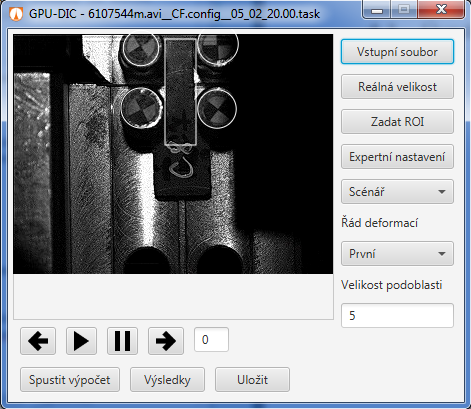
\includegraphics[width=0.5\textwidth]{hlavniOkno.png}\\Hlavní okno programu}
\end{figure}
\begin{description}
\item[Vstupní soubor] načte vstupní souboru(y), podporovány jsou videa (*.avi), obrázky (*.bmp, *.jpg), konfigurace úlohy (*.config), soubor projektu (*.task) a skript pro více úloh (*.scr)
\item[Reálná velikost] otevře okno pro vyznačení známého rozměru v obraze
\item[Zadat ROI] otevře okno pro vyznačení ROI
\item[Exporty] otevře okno pro specifikaci exportů provedených po dokončení výpočtu
\item[Velikost facetu] slouží pro zadání velikosti facetu použitou během výpočtu
\item[Expertní nastavení] slouží pro nastavení specifických parametrů enginu
\item[Šipky] slouží pro prohlížení obrázků
\item[Spustit výpočet] spustí výpočet
\item[Výsledky] otevře okno pro prezentaci výsledků (dostupné po dokončení výpočtu)
\item[Uložit] otevře dialog pro uložení skriptu úlohy dle konkrétního nastavení a pro uložení celého projektu (včetně výsledků)        
\end{description}
\newpage
\subsection{Načtení vstupu}
\begin{description}
\item[Video] soubor musí mít koncovku avi, video se rozseká na obrázky za pomoci programu VirtualDub 
\item[Obrázky] se řadí dle přirozeného třídění (tj. většinou dle abecedy)
\item[Config] soubor je textový soubor obsahující konfiguraci výpočtu, typicky po načtení může být rovnou spuštěn výpočet
\item[Task] soubor obsahuje kromě konfigurace úlohy také vypočtené výsledky, které lze okamžitě po načtení souboru prohlížet
\item[Scr] soubor by měl obsahovat seznam konfigurací, které se mají spočítat. Cesty ke konfiguracím musí být v absolutním tvaru (např. C:\textbackslash temp\textbackslash prvni.config), každá na samostatném řádku
\end{description}
Aplikace je schopna zobrazovat reálný čas děje, je ale nutné, aby ve složce, kde se nachází vstup, byl i ".uda" soubor s informací o fps analyzovaného videa. Pokud nebyl automaticky vygenerován kamerou, je možno ho ručně vytvořit. Jedná se o prostý textový soubor, ve který by měl být řádek ve tvaru "Speed = 5000fps," kde číslo 5000 se nahradí počtem snímků za vteřinu daného vstupu.
\newpage
\subsection{Zadávání ROI}
\begin{figure}[H]
\center{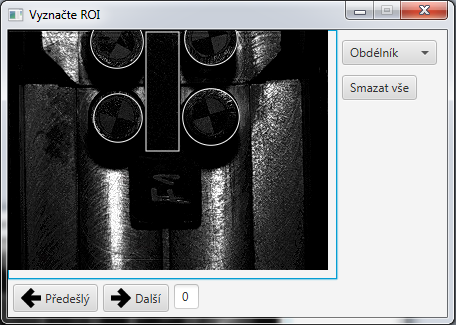
\includegraphics[width=0.5\textwidth]{ROI.png}\\Okno pro vyznačení ROI}
\end{figure}
Zadáním ROI může uživatel enginu říci, které oblasti má počítat a tím pádem dost urychlit výpočet. Dostupné tvary ROI jsou obdélník a kruh. Na výběr jsou dvě možnosti vyznačení. První je statické umístění ROI (v téměř libovolném počtu). Tyto ROI se budou dodržovat po celou dobu výpočtu, případně je možno specifikovat na různá kola různá ROI s tím, že pokud nejsou uvedena jiná ROI, použijí se ROI z předchozího kola (takže pokud nás zajímá pouze jedna oblast během celého výpočtu, stačí ji označit pro první kolo).\\
Druhou možností je vyznačení polohy čelistí za pomoci 4 kruhových ROI (odtud pochází omezení na ne zcela libovolný počet statických ROI). V tomto případě se engine pokusí automaticky sledovat čelisti a podle toho upravuje sledovanou oblast. Sledovaná oblast může být v tomto případě definována dvěma způsoby - buď ji uživatel vyznačí sám za pomoci obdélníkové oblasti nebo vyznačení nechá na enginu. Engine vytvoří oblast dle jednoduchých pravidel - oblast je mezi čelistmi, začíná nad horními čelistmi a končí pod spodními čelistmi s tím, že se nechává mezera mezi čelistí a sledovanou oblastí pro alespoň částečné potlačení nepřesnosti vyznačení čelistí a tím pádem ovlivnění výpočtu.\\
Vlastní vyznačení se děje za pomoci kliknutí a tažení levým tlačítkem myši. Pokud uživatel není spokojen s umístěním oblasti, je možno ji chycením a tažením přemisťovat. Pravým tlačítkem myši pak lze danou oblast vymazat.
\newpage
\subsection{Exporty výsledků}
\begin{figure}[H]
\center{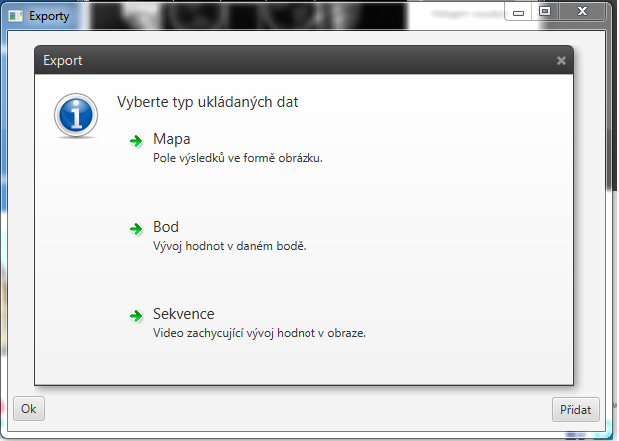
\includegraphics[width=0.5\textwidth]{initialExport.png}\\Možnosti exportů}
\end{figure}
Před výpočtem je možno zadat exporty, které se provedou po dokončení výpočtu. V tomto kroku se nevybírá konkrétní kolo (obrázek), pro který se export bude provádět, daný export se provede vždy pro všechna kola. Vybíráme tedy pouze formát a směr (typ) exportovaných dat. Výstupní formáty jsou k dispozici tři - obrázek (mapa), csv (textový export výsledků) nebo video (animace vývoje hodnot). Směr (či typ) dat určuje jednak, jestli se bude jednat o výsledná posunutí nebo přetvoření, a také směr dané hodnoty (pro posunutí X, Y nebo absolutní hodnota. u přetvoření pak XX, XY, YY a absolutní hodnota). Názvy výstupních souborů jsou pak generovány automaticky z parametrů úlohy (detaily lze nalézt v kapitole \ref{sec:names}).
\newpage
\subsection{Názvy výstupních souborů}
\label{sec:names}
\begin{description}
\item [Task soubor] [název]\textunderscore [vf].task
\item [Config soubor] [název]\textunderscore [vf].config
\item [Posuny čelistí] [název]\textunderscore [vf].csv
\item[Obrazová mapa hodnot]  [název]\textunderscore [čas]\textunderscore [typ]\textunderscore [vf].bmp
\item[Textová mapa hodnot] [název]\textunderscore [pos]\textunderscore [vf].csv
\item[Vývoj hodnot v bodě] [název]\textunderscore [čas]\textunderscore [typ]\textunderscore [vf].csv
\item[Video] [název]\textunderscore [typ].avi
\end{description}
\begin{center}\textbf{Legenda:}\end{center}
\begin{description}
\item[název] Jméno vstupního souboru (nemusí nutně být název videa, může to být např. název config souboru)
\item[vf] velikost facetu
\item[čas] čas, ve kterém dané výsledky platí či ve kterém se udály  
\item[typ] směr (typ) výsledků 
\item[pos] pozice výsledku (X a Y)
\end{description}
\newpage
\subsection{Vyznačení reálné velikosti}
\begin{figure}[H]
\center{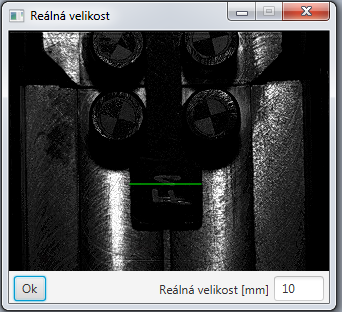
\includegraphics[width=0.5\textwidth]{realSize.png}\\Okno pro vyznačení reálné velikosti}
\end{figure}
Konfigurace úlohy z hlediska fyzického uspořádání se může měnit, pro porovnávání výsledků by bylo dobré mít možnost zadávat parametry pro engine v reálných jednotkách. Pixely nejsou tolik vhodné, protože jeho rozměr se může vlivem změny vzdálenosti kamery a vzorku lišit. Proto je k dispozici okno pro vyznačení známého rozměru v obraze spolu se zadáním jeho reálné délky, což umožní spočítat převodní koeficient px / mm, který se využívá pro stanovení velikosti okna při výpočtu pole přetvoření. Tím lze zajistit stejné vlastnosti algoritmu (hlavně vyhlazení / vynechání detailů) pro různá uspořádání.\\
Proces vyznačení je prostý, uživatel vyznačí známý horizontální rozměr za pomoci kliknutí levého tlačítka myši a tažením a vyplní jeho délku v milimetrech. Program ulehčuje práci tím, že umožňuje vyznačit pouze horizontální čáru, takže uživatel nemusí řešit, jestli je čára skutečně rovná. Pokud uživatel chce nakreslit čáru znovu, stačí pouze znovu vyznačit za pomoci levého tlačítka, stará linie se automaticky smaže.
\subsection{Expertní nastavení}
\begin{figure}[H]
\center{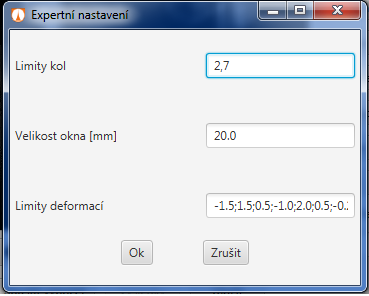
\includegraphics[width=0.5\textwidth]{expert.png}\\Expertní nastavení}
\end{figure}
V tomto okně lze nastavit detailní parametry enginu, většinu z nich není v běžném případě nutné nastavovat. V této sekci nebudou jednotlivé volby popisovány, pouze bude uveden jejich systémový název, který lze dohledat v kapitole \ref{sec:parameters}, kde je uveden i jejich podrobný popis.
\begin{description}
\item[Varianta generátoru] FACET\textunderscore GENERATOR\textunderscore METHOD
\item[Parametr generování] FACET\textunderscore GENERATOR\textunderscore PARAM
\item[Varianta rozdělení] TASK\textunderscore SPLIT\textunderscore METHOD
\item[Parametr rozdělení] TASK\textunderscore SPLIT\textunderscore PARAM
\item[Kernel] KERNEL
\item[Interpolace] INTERPOLATION
\item[Limity kol] ROUND\textunderscore LIMITS
\item[Velikost okna] STRAIN\textunderscore ESTIMATION\textunderscore PARAM
\item[Limity deformací] DEFORMATION\textunderscore LIMITS 
\end{description}
\subsection{Spuštění výpočtu}
Spuštění výpočtu neobnáší nic zvláštního, stačí pouze kliknout na tlačítko. Nenastavené parametry enginu (prakticky pouze hodnoty z expertního nastavení) se nastaví na výchozí hodnoty, které by měly být vhodné pro drtivou většinu záznamů trhacích zkoušek (konkrétní hodnoty lze nalézt v kapitole \ref{sec:parameters}).
\subsection{Uložení}
\begin{figure}[H]
\center{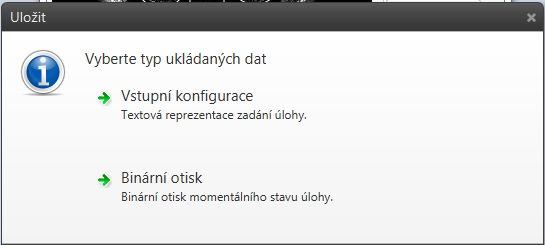
\includegraphics[width=0.5\textwidth]{saveCfgBin.png}\\Uložení projektu}
\end{figure}
Úlohu lze uložit dvěma způsoby - jako textovou konfiguraci či binární otisk. Textová konfigurace se hodí v případě, že chcete opakovat výpočet nebo spustit více výpočtů po sobě za pomoci skriptu. Uložený soubor obsahuje všechny nastavené parametry výpočtu, takže po jeho načtení se může rovnou spouštět výpočet. Binární otisk úlohy také uloží nastavení úlohy, uloží také vypočtené výsledky, takže je možno je prohlížet i později (binární otisk se automaticky ukládá vždy po dokončení výpočtu).
\newpage
\subsection{Výsledky}
\begin{figure}[H]
\center{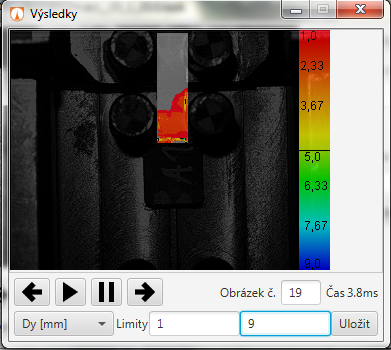
\includegraphics[width=0.5\textwidth]{results.png}\\Okno s výsledky}
\end{figure}
Okno výsledků prezentuje mapy s vypočtenými výsledky. Jsou dostupné jak kumulativní výsledky, tak diferenciální (ty mají před názvem písmeno "d"). Kromě prohlížení výsledků je také možno výsledky exportovat. K dispozici je export právě zobrazené mapy nebo celé sekvence map. Mapy lze exportovat buď jako obrázek (obdoba obrázku v okně), nebo jako seznam hodnot do souboru CSV. Kromě exportu po jednotlivých mapách lze také vytvořit animaci, která vytvoří video soubor prezentující zvolené výsledky jako video. Názvy výsledných souborů se generují automaticky dle klíče, který lze nalézt v kapitole \ref{sec:names}.
\begin{figure}[H]
\center{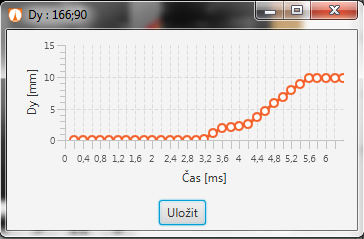
\includegraphics[width=0.5\textwidth]{resultsPoint.png}\\Výsledky pro bod}
\end{figure}
Kliknutím do obrázku je možno zobrazit vývoj vybrané hodnoty v daném bodě. Vývoj hodnoty je reprezentován grafem, kde na horizontální ose je čas a na vertikální sledovaná veličina. Typ zobrazené hodnoty se automaticky aktualizuje vzhledem k vybrané hodnotě v hlavním okně s výsledky. Tlačítkem "Uložit" je možné uložit zobrazené hodnoty do CSV souboru (jméno souboru se generuje automaticky ze souřadnic bodu, typu dat a nastavení úlohy). Je možno mít otevřeno několik oken s různými body najednou.
\newpage
\section{Doporučená nastavení}
\label{sec:goodSettings}
\begin{description}
\item[Velikost facetu] Vzhledem k šumu ve videu je vhodné volit velikost facetu minimálně 20, příliš vysoké hodnoty ale mohou způsobit ignorování detailů, není tedy vhodné překročit hodnotu cca 30. Je také nutné dbát na to, aby generovaný facet nebyl větší než sledovaná oblast, v tom případě by skoro určitě docházelo ke zkreslení výsledků vlivem zahrnutí pozadí do sledování.
\item[Velikost okna] Tento parametr by měl nejlépe korespondovat se zvolenou velikostí facetu, případně může být větší. Hodnota menší než velikost facetu nemá příliš smysl, protože detaily jsou ignorovány díky zvolené velikosti facetu a promítnou se do pole posunutí, ze kterého se počítá pole přetvoření. Je nutné ale dát pozor na to, že tato velikost se zadává v milimetrech, zatímco velikost facetu je v pixelech.
\item[ROI] Nevhodnější je použít variantu dynamického výpočtu, tj. vyznačit pozice čelistí. Algoritmus pak na základě polohy čelistí vytvoří oblast materiálu a také se postará o posouvání oblastí dle detekovaného pohybu čelistí. 
\item[Limity kol] Algoritmus vynechá výpočet deformací v případě, že detekuje nulový pohyb čelistí. Není tedy nezbytně nutné limity kol definovat, mohou se hodit v případě, že nás zajímá pouze konkrétní část videa, ne celý děj.
\end{description}
\newpage
\section{Parametry enginu}
\label{sec:parameters}
V této kapitole budou uvedeny parametry enginu, které lze měnit (ať už za pomoci GUI či konfiguračního souboru) spolu s popisem, jaké hodnoty lze použít. Za názvem parametru bude v hranaté závorce uvedena stručná charakteristika povolené hodnoty (int - celé číslo, double - reálné číslo, výčet povolených hodnot pro některé parametry, výchozí hodnota pak bude zvýrazněna \textbf{tučně}).
\begin{description}
\item[FACET\textunderscore GENERATOR\textunderscore METHOD] [CLASSIC | \textbf{TIGHT}]\\
Způsob generování facetu. CLASSIC používá klasický režim generování, kde se facety pokládají vedle sebe s malým přesahem. Tento režim je vhodný pro deformace typu posunutí (tento režim se používá pro sledování posunu čelistí), v případě složitějších deformací nemusí být výsledné pole posunů homogenní. TIGHT klade facety přes sebe s malou mezerou, což vylepší homogenitu výsledného pole a lépe odolá šumu, daní je ale mnohem vyšší počet facetů a tím pádem i mnohem delší výpočet. Ve výchozím stavu se používá TIGHT režim.
\item[FACET\textunderscore GENERATOR\textunderscore PARAM] [int]\\
Parametr generování úzce souvisí se způsobem generování. Pro CLASSIC režim tento parametr určuje kolik pixelů z facetů se bude překrývat. V TIGHT režimu parametr určuje o kolik se posune okraj následujícího facetu oproti předchozímu. Výchozí hodnotou je 1. Je nutné dát pozor na jistá omezení hodnot, které vycházejí z principu generování facetů. V CLASSIC režimu má parametr smysl pro hodnoty maximálně do velikosti facetu, poté už se nové facety umisťují špatně nebo výsledný počet facetu je nekonečný. V případě TIGHT režimu musí být hodnota kladné číslo, nulová hodnota by způsobila nekonečně mnoho facetů, záporné hodnoty by způsobily generování facetů na špatné pozici.
\item[FACET\textunderscore SIZE] [int]\\
Tento parametr je velikost facetu. Doporučené hodnoty lze nalézt v kapitole \ref{sec:goodSettings}.
\item[KERNEL] [CL\textunderscore 2D\textunderscore I | CL\textunderscore 1D\textunderscore I\textunderscore V\textunderscore LL\textunderscore MC | \textbf{CL\textunderscore 1D\textunderscore I\textunderscore V\textunderscore LL\textunderscore MC\textunderscore D}]\\
Typ OpenCL kernelu, který bude použit pro výpočet na GPU. Výchozí a doporučená hodnota je CL\textunderscore 1D\textunderscore I\textunderscore V\textunderscore LL\textunderscore MC\textunderscore D, ostatní jsou vhodné pouze pro testovací režim nebo některé speciální případy. Pro kernely jiné než výchozí není garantována stabilita programu.
\item[TASK\textunderscore SPLIT\textunderscore METHOD] [NONE | STATIC | \textbf{DYNAMIC}]\\
Vzhledem k omezenému množství paměti na GPU je někdy nutné rozdělit úlohu na menší části. Varianta NONE zakáže rozdělování úlohy. To lze úspěšně použít pouze pro malé úlohy, v ostatních případech výpočet spadne. STATIC umožní definovat, po kolika facetech se má úloha rozdělit. Tato varianta se může hodit v případě, kdy nechcete plně vytěžovat paměť GPU. Poslední varianta DYNAMIC se pokusí co možná nejvíce zaplnit paměť GPU daty, což je z hlediska délky výpočtu nejefektivnější, protože se minimalizují přenosy dat z / do GPU a díky tomu to je také výchozí hodnota.
\item[TASK\textunderscore SPLIT\textunderscore PARAM] [int]\\
NONE a DYNAMIC rozdělování úlohy parametr nevyžadují, u varianty STATIC je nutné stanovit počet facetů tvořících jednu pod-úlohu. Výchozí hodnota je 1000, celková velikost úlohy ale také dost závisí na počtu testovaných deformací, takže nelze stanovit nějaké univerzální pravidlo, vesměs je nutno postupovat způsobem pokus-omyl, dokud nedosáhneme požadované paměťové náročnosti.
\item[INTERPOLATION] [BILINEAR | \textbf{BICUBIC}]\\
Po deformaci facetu jsou souřadnice bodů facetu obecně reálná čísla, je tedy nutné nějakým způsobem zasadit bod zpět do rastru obrazu a získat jeho barvu. K tomu se používá proces interpolace barvy. Volba BILINEAR používá lineární interpolaci v ploše, zatímco BICUBIC používá kubickou funkci pro dopočet výsledné barvy. BICUBIC varianta by měla produkovat kvalitnější výsledky, je ale také náročnější na výpočet.
\item[ROUND\textunderscore LIMITS] [int ; int]\\
Limity kol je možné stanovit k urychlení výpočtu (např. pro vynechání části záznamu, kde již došlo k přetržení vzorku). Hodnoty se zadávají ve formě indexů prvního a posledního snímku (číslováno od 0), čísla se oddělují středníkem.
\item[RESULT\textunderscore QUALITY] [double]\\
Deformace se odhaduje na základě míry korelace barev pixelů původního a deformovaného facetu. Čím vyšší je tato hodnota, tím pravděpodobněji se jedná o správný odhad. Maximální hodnotu je pak 1.0, což znamená, že se vstup a výstup se naprosto shodují. Vlivem šumu a diskretizací prostoru možných deformací se ale maximální hodnoty prakticky nikdy nedosáhne, pouze se jí můžeme přiblížit. Často máme pro jeden pixel několik možných výsledků, což umožní částečně eliminovat vliv šumu na výsledek. Tento parametr říká, jak moc kvalitní musí být výsledek, aby byl přijat do skupiny výsledných. Výchozí hodnota je 0.5, což zaručuje vynechání nekvalitních výsledků při zachování dostatečného počtu výsledků pro úspěšný výsledek. 
\item[STRAIN\textunderscore ESTIMATION\textunderscore PARAM] [double]\\
Tento parametr určuje velikost okna při výpočtu pole přetvoření. Tento parametr se zadává v mm, engine si pak velikost v pixelech dopočítá sám za pomoci parametru MM\textunderscore TO\textunderscore PX\textunderscore RATIO.
\item[MM\textunderscore TO\textunderscore PX\textunderscore RATIO] [double]\\
Koeficient pro přepočet rozměru okna přetvoření z milimetrů na pixely. Jedná se o hodnotu, která říká, kolik pixelů v obraze je jeden milimetr v reálném světě.
\item[DEFORMATION\textunderscore LIMITS] [double ; double ; double...]\\
Limity deformací určují, jaké deformace se v obraze předpokládají a tím pádem jaké deformace se budou testovat. Hodnoty se pro každý koeficient zadávají ve tvaru MIN, MAX, KROK, koeficienty mohou být dva (testovat se budou pouze posuny), 6 (kromě posunutí také prodloužení a smyk) nebo 12 (přidají se nelineární deformace). Tím pádem se musí zadat 6, 18 nebo 36 hodnot oddělených středníkem. Matematické využití koeficientů lze nalézt v přiložené literatuře. Jako výchozí hodnota se používají deformace prvního řádu s následujícím zadáním : -1; 1; 0.5; -2; 5; 0.5; -0.0; 1.0; 0.1; -0.5; 0.5; 0.1; -0.5; 0.5; 0.1; -0.0; 1.0; 0.1. V překladu jde o to, že posuny se testují po 0.5 pixelech, v ose X se testují pouze malé posuny. Deformace prvního řádu pak testují prodloužení od žádného (0) do prodloužení na dvojnásobek (1) jak v ose X, tak Y, a smyk pak záporný i kladný v obou osách (-0.5 až 0.5). Vliv koeficientů na deformaci lze vyzkoušet v přiloženém nástroji \emph{DIC\textunderscore DeformationGenerator} (ovládání programu je popsáno v kapitole \ref{sec:generator}).
\end{description}
\newpage
\section{Konfigurační soubor úlohy}
\label{sec:config}
Konfigurační soubor v běžném případě není nutné psát ručně, lze ho vygenerovat v aplikaci po nastavení všeho potřebného, ukázkový soubor lze nalézt v kapitole \ref{sec:configExample}. Soubor je textový, každý parametr je uveden na samostatném řádku. Parametr se skládá z identifikátoru (název velkými písmeny), oddělovače (ten je tvořen dvojnásobnou dvojtečkou - "::") a hodnotou parametru.\\
Povinným parametrem je vstupní soubor. Tím může být buď cesta k video-souboru (cesta musí být absolutní) nebo seznam obrázků ke zpracování, názvy pak musí být odděleny středníkem. Název parametru pro vstupní soubor je pak "INPUT."\\
Dále je možno stanovit ROI pro jednotlivá kola. Identifikátor je "ROI\textunderscore " a číslo obrázku (např. ROI\textunderscore 0 pro první obrázek). Hodnotou je pak výčet ROI pro dané kolo oddělených dvojitými středníky. ROI se definuje jako posloupnost hodnot (souřadnice ROI -- limity deformací -- velikost facetu) oddělených dvojitou pomlčkou ("--"). Souřadnice ROI mohou být buď souřadnice středu a poloměr (pro kruhový ROI) nebo souřadnice levého horního a pravého spodního bodu (obdélníkový ROI, v pořadí X1;Y1;X2;Y2), jednotlivé hodnoty jsou od sebe odděleny středníkem. Limity deformací se specifikují ve stejném tvaru jako globální limity (viz. kapitola \ref{sec:parameters}), případně lze uvést slovo "NONE", které specifikuje, že se mají použít limity globální. Obdobně se chová velikost facetu, celočíselná hodnota určí velikost, NONE vynutí použití globálního nastavení.\\
Dále lze v souboru nastavit i parametry enginu. Identifikátor parametru se tvoří jako klíčové slovo "PARAM\textunderscore" následované názvem parametru (např. PARAM\textunderscore FACET\textunderscore SIZE), hodnota se pak musí řídit možnostmi hodnot daného parametru (opět viz. kapitola \ref{sec:parameters}). Všechny neuvedené hodnoty budou nahrazeny výchozí hodnotou - nemusí se tedy nutně specifikovat každý parametr, pouze ty, které chceme změnit.\\
V ukázkách lze nalézt dva soubory. První je dalo by se říci minimalistický - obsahuje minimální počet parametrů pro úspěšný výpočet. Vstupem je video, ROI jsou čtyři kružnice označující pozici čelistí (což zajistí inteligentní posunovaní jak ROI čelistí, tak automatické vytvoření ROI vzorku) a velikost facetu. Je nutné dát pozor na zápis ROI, který se bohužel nevejde na jeden řádek a je tudíž zalomen. V reálném souboru je ale nutné dodržet, aby ROI pro dané kolo byly všechny napsány na jednom řádku (čili v ukázce se jedná o jeden dlouhý řádek rozdělený na několik).\\
Druhá ukázka pak představuje plnou konfiguraci, ukazuje i definici ROI pro jednotlivá kola - druhé kolo má obdélníkový ROI používající specifikované limity deformací (pouze posuny) při velikosti facetu 25, zatímco ve třetím kole se použijí výchozí hodnoty jak pro limity, tak pro velikost facetu.
\newpage
\section{Ukázky konfiguračních souborů}
\label{sec:configExample}
\begin{lstlisting}[title=Jednoduchý konfigurační soubor pro automatický výpočet]
INPUT :: D:\temp\7202845m\7202845m.avi
ROI_0 :: 110.0;88.0;24.20--NONE--NONE;; 203.0;9.0;26.24--NONE--NONE;; 203.0;87.0;28.28--NONE--NONE;; 109.0;12.0;26.24--NONE--NONE
PARAM_FACET_SIZE :: 20
\end{lstlisting}
\begin{lstlisting}[title=Plný konfigurační soubor pro automatický výpočet]
INPUT :: D:\temp\7202845m\7202845m.avi
ROI_2 ::  100.0;100.0;150.0;150.0---2.0,,2.0,,0.1,,-5.0,,10.0,,0.1--25
ROI_3 ::  109.0;109.0;159.0;159.0---NONE--NONE
PARAM_FACET_GENERATOR_METHOD :: TIGHT
PARAM_FACET_GENERATOR_PARAM :: 1
PARAM_FACET_SIZE :: 20
PARAM_KERNEL :: CL_1D_I_V_LL_MC_D
PARAM_TASK_SPLIT_METHOD :: DYNAMIC
PARAM_INTERPOLATION :: BICUBIC
PARAM_ROUND_LIMITS :: 2;4
PARAM_DEFORMATION_LIMITS :: -1.0;1.0;0.1;-2.0;5.0;0.1
\end{lstlisting}
\newpage
\section{Ovládání programu DIC\textunderscore DeformationGenerator}
\label{sec:generator}
\begin{figure}[H]
\center{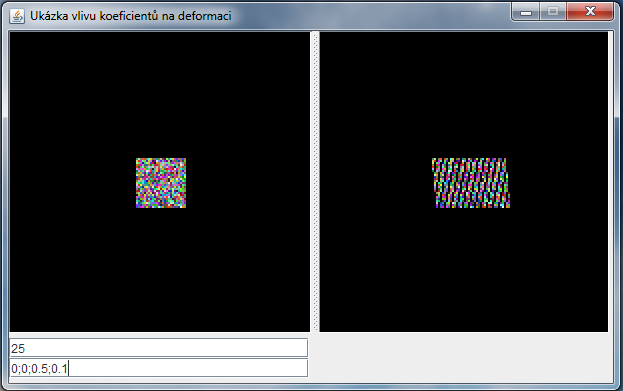
\includegraphics[width=0.5\textwidth]{defGen.png}\\Okno programu}
\end{figure}
Program slouží pro demonstraci vlivu koeficientů na deformaci facetu. V horní části jsou dva obrázky - levý prezentuje původní stav facetu (barevný vzor se generuje náhodně při změně velikosti facetu), vpravo je pak stav po deformaci. Pod obrázky jsou dvě vstupní pole - první určuje velikost facetu, druhá pak koeficienty deformace. Koeficienty deformace se zapisují jako sekvence reálných čísel oddělených středníky (oddělovač desetinných míst záleží na nastavení OS, typicky je to tečka. Lze to poznat tak, že po zadání koeficientu se výstup nezmění). Není nutné vypisovat přesný počet koeficientů dle zvoleného řádu (2, 6 nebo 12), stačí napsat koeficienty, které nás zajímají. Hodnoty není potřeba potvrzovat, data se generují okamžitě po napsání znaku.
\end{document}